%%%%%%%%%%%%%%%%%%%%%%%%%%%%%%%%%%%%%%%%%%%%%%%%%%%%%%%%%%%%%%%%%
\begin{frame}[fragile]
\frametitle{\textbf{\textcolor{orange}{Taylor shift by $1$ execution times}}}

\textcolor{blue}{\textbf{Results are for polynomials of sizes $n=2^e$ :}}

\begin{center}
\tiny{
\begin{tabular}{||c|c||c||r|r||r||}
   \hline
  \multicolumn{6}{||c||}{\textbf{Execution time in seconds}} \\
 \hline
  e  &    n    &    GPU     &  CPU : HOR  &   CPU : DNC  &  Maple 16   \\  \hline \hline
  3  &      8  &  0.001518  &   0.000128  &    0.000141  &     <0.001  \\
  4  &     16  &  0.001432  &   0.000186  &    0.000172  &     <0.001  \\
  5  &     32  &  0.001590  &   0.000167  &    0.000191  &     <0.001  \\
  6  &     64  &  0.001773  &   0.000192  &    0.000294  &      0.008  \\
  7  &    128  &  0.002016  &   0.000261  &    0.000628  &      0.024  \\
  8  &    256  &  0.003036  &   0.000593  &    0.002331  &      0.084  \\
  9  &    512  &  0.002624  &   0.001278  &    0.006304  &      0.320  \\
 10  &   1024  &  0.005756  &   0.005940  &    0.032073  &      1.400  \\
 11  &   2048  &  0.009317  &   0.015312  &    0.095027  &      5.640  \\
 12  &   4096  &  0.013475  &   0.076866  &    0.376543  &     24.478  \\
 13  &   8192  &  0.019674  &   0.324029  &    1.498890  &    104.438  \\
 14  &  16384  &  0.027229  &   1.282708  &    6.861433  &    437.848  \\
 15  &  32768  &  0.042561  &   5.110919  &   23.907799  &   1781.427  \\
 16  &  65536  &  0.064306  &  15.184347  &  114.988129  &   7407.063  \\
 17  & 131072  &  0.127214  &  80.625801  &  477.934692  &     >10000  \\
   \hline 
\end{tabular}
}
\end{center}

\end{frame}
%%%%%%%%%%%%%%%%%%%%%%%%%%%%%%%%%%%%%%%%%%%%%%%%%%%%%%%%%%%%%%%%%

%%%%%%%%%%%%%%%%%%%%%%%%%%%%%%%%%%%%%%%%%%%%%%%%%%%%%%%%%%%%%%%%%
\begin{frame}[fragile]
\frametitle{\textbf{\textcolor{orange}{Execution time of the GPU in function of $e$}}}

\begin{center}
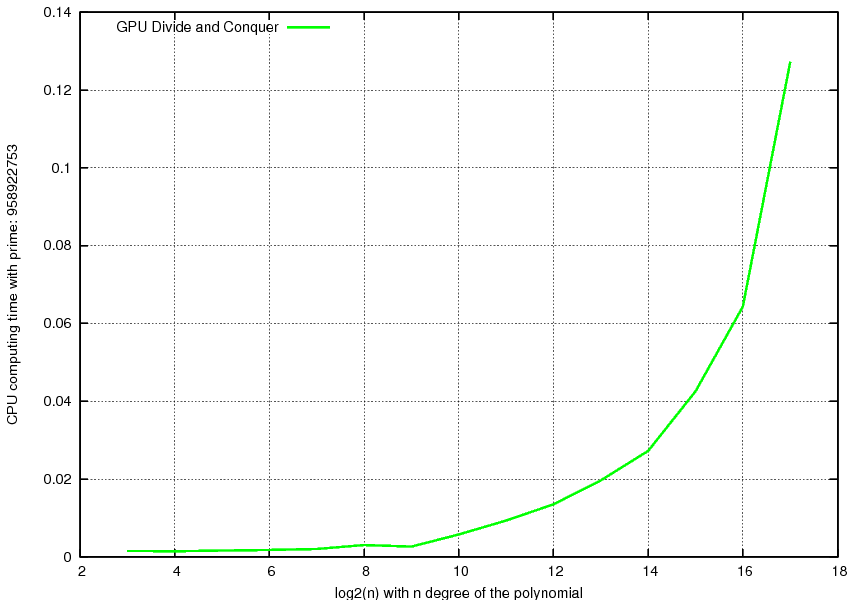
\includegraphics[scale=0.25]{eps/GPUtime_e.png}\\
%\textbf{Execution time of the GPU in function of $e$}\\
\end{center}

\end{frame}
%%%%%%%%%%%%%%%%%%%%%%%%%%%%%%%%%%%%%%%%%%%%%%%%%%%%%%%%%%%%%%%%%

%%%%%%%%%%%%%%%%%%%%%%%%%%%%%%%%%%%%%%%%%%%%%%%%%%%%%%%%%%%%%%%%%
\begin{frame}[fragile]
\frametitle{\textbf{\textcolor{orange}{Execution time of the GPU in function of $n$}}}

\begin{center}
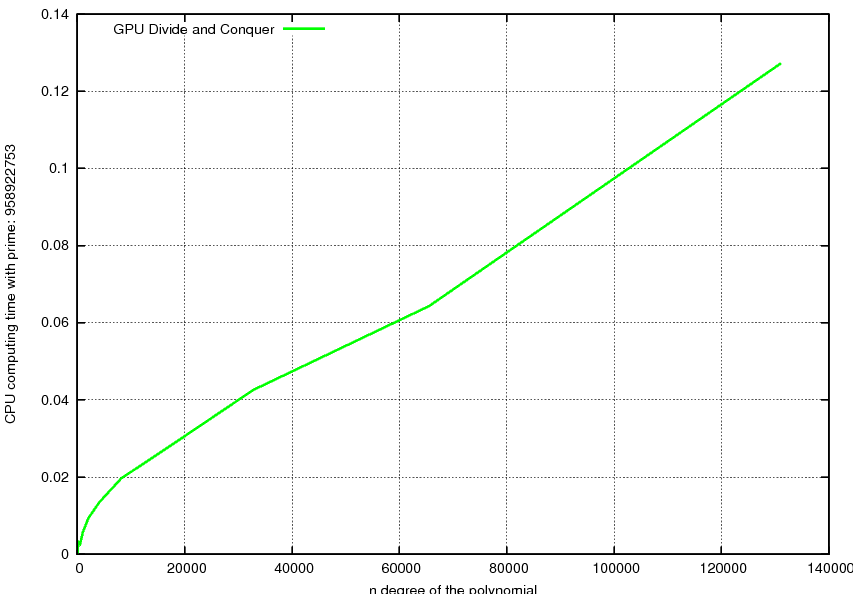
\includegraphics[scale=0.25]{eps/GPUtime_n.png}\\
%\textbf{Execution time of the GPU in function of $n$}\\
\end{center}

This execution time is approximatively linear.

\end{frame}
%%%%%%%%%%%%%%%%%%%%%%%%%%%%%%%%%%%%%%%%%%%%%%%%%%%%%%%%%%%%%%%%%

%%%%%%%%%%%%%%%%%%%%%%%%%%%%%%%%%%%%%%%%%%%%%%%%%%%%%%%%%%%%%%%%%
\begin{frame}[fragile]
\frametitle{\textbf{\textcolor{orange}{Execution times of the CPU in function of $n$}}}

\begin{center}
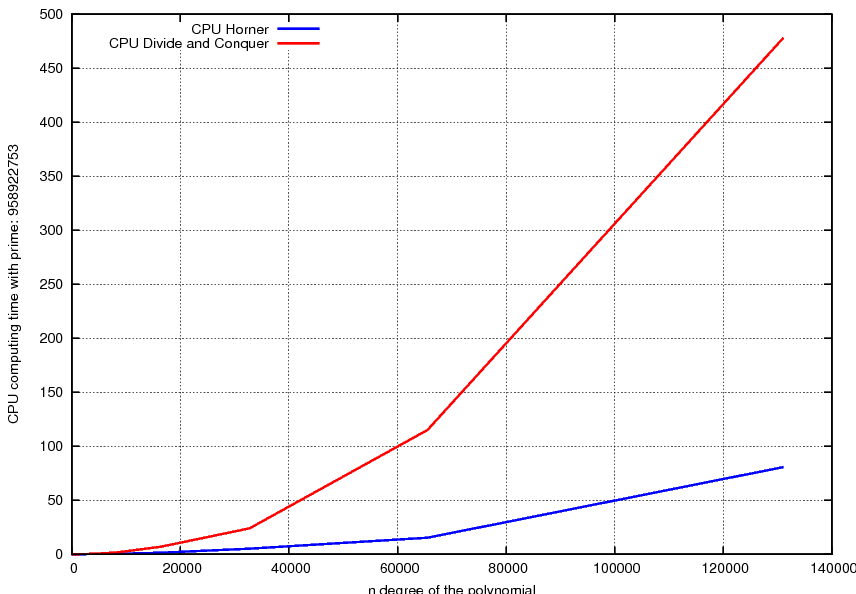
\includegraphics[scale=0.25]{eps/CPUtime_n.png}\\
\end{center}


\end{frame}
%%%%%%%%%%%%%%%%%%%%%%%%%%%%%%%%%%%%%%%%%%%%%%%%%%%%%%%%%%%%%%%%%

%%%%%%%%%%%%%%%%%%%%%%%%%%%%%%%%%%%%%%%%%%%%%%%%%%%%%%%%%%%%%%%%%
\begin{frame}[fragile]
\frametitle{\textbf{\textcolor{orange}{Execution times in function of $n$ for small degrees}}}

\begin{center}
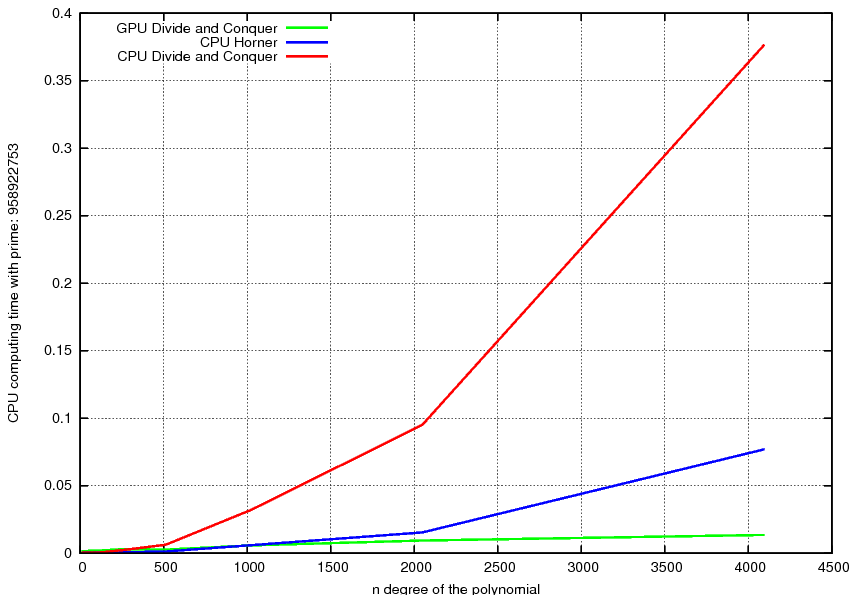
\includegraphics[scale=0.25]{eps/time_small_n.png}\\
\end{center}

\end{frame}
%%%%%%%%%%%%%%%%%%%%%%%%%%%%%%%%%%%%%%%%%%%%%%%%%%%%%%%%%%%%%%%%%

%%%%%%%%%%%%%%%%%%%%%%%%%%%%%%%%%%%%%%%%%%%%%%%%%%%%%%%%%%%%%%%%%
\begin{frame}[fragile]
\frametitle{\textbf{\textcolor{orange}{Execution times in function of $n$ for big degrees}}}

\begin{center}
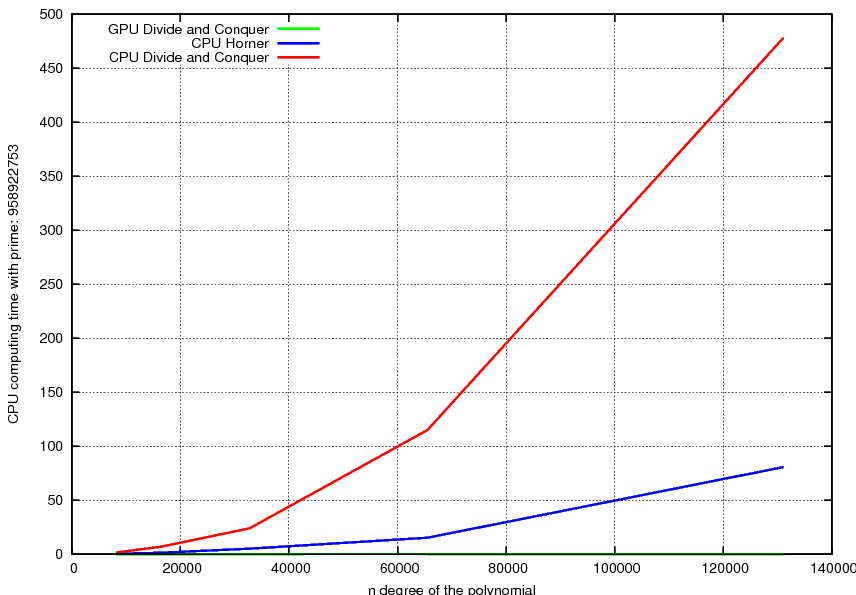
\includegraphics[scale=0.25]{eps/time_big_n.png}\\
\end{center}

We clearly improve performances using GPUs.\\
\textcolor{darkgreen}{\textbf{Remark :}} the behaviour of the CPU times is the same for the different sizes.

\end{frame}
%%%%%%%%%%%%%%%%%%%%%%%%%%%%%%%%%%%%%%%%%%%%%%%%%%%%%%%%%%%%%%%%%
